% ch2p15_002: Specifying coordinates
% Draw cosine line from the end of sine line
\documentclass[tikz, border=10pt]{standalone}

\usepackage{tikz}

\begin{document}
	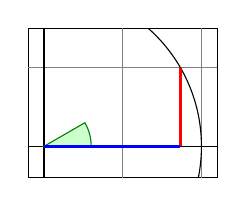
\begin{tikzpicture}[scale=2]
		\clip[draw] (-0.1, -0.2) rectangle (1.1, 0.75);
		
		\draw[step=0.5cm, gray, very thin] (-1.4, -1.4) grid (1.4, 1.4);
		\draw (-1.5, 0) -- (1.5, 0); % x-axis
		\draw (0, -1.5) -- (0, 1.5); % y-axis
		\draw (0, 0) circle [radius=1cm];
		
		\filldraw[fill=green!20, draw=green!50!black] (0, 0) -- (3mm, 0mm)
		arc [start angle=0, end angle=30, radius=3mm] -- cycle;
		
		% sine line
		% (30:1cm) -- Given in polar co-ordinates
		%     means 30 degrees and 1cm radius
		% End point of the line will be 
		%     (30:1cm) converted to cartesian co-ordinates
		%     and added to (0, -0.5). And the end point 
		%     touches the x-axis.
		\draw[red, very thick] (30:1cm) -- +(0, -0.5);
		
		% Cosine line
		% (30:1cm) ++(0, -0.5) ==> Results in a coordinate where sine line ends. And we are ending the cosine line at (0, 0).
		\draw[blue, very thick] (30:1cm) ++(0, -0.5) -- (0, 0);
	\end{tikzpicture}
\end{document}